\section{Trigonometric Functions}
\label{sec:funzioni_trigonometriche}%

Consider the unit circle 
\[
  U = \ENCLOSE{z\in \CC\colon \abs{z} = 1}.
\]
Each point $z\in U$ determines a geometric angle with the real axis.
Our objective is now to define the measure of an angle.
The point $z=1$ will determine an angle of zero measure, and 
by rotating $z$ counterclockwise, we want to obtain angles 
of increasing measure such that the angle obtained 
by juxtaposing one after the other the angles determined 
by the point $z$ and the point $w$ has a measure equal to the sum of the
measures
of the angles determined by $z$ and $w$.

We arbitrarily choose to assign a measure $\tau>0$ to the full angle.
The intuitive idea is to \emph{wrap} the line $\RR$ like a thread 
around the circle $U\subset \CC$ 
by mapping the point $0\in \RR$ to the point $1\in \CC$,
then the point $\frac \tau 4$ to $i$, the point $\frac \tau 2$ to $-1$,
the point $3\frac \tau 4$ to $-i$, and the point $\tau$ back to $1$.
Intermediate points will map to intermediate points of $U$ in such a way as to
have
the additivity of angles: the measure of the sum of two angles must 
be the sum of the measures.

The set $U$ inherits the multiplicative group structure of $\CC$: 
if $z,w\in U$, 
then $z\cdot w \in U$ since $\abs{z\cdot w} = \abs{z}\cdot \abs{w} = 1$
given that $\abs{z}=\abs{w}=1$.
Recall also that the multiplication of unit complex numbers 
corresponds to the sum of their geometric angles.
Thus, the function $\phi\colon \RR \to U$ that measures the angles 
must have the property of a \emph{homomorphism}:
\begin{equation}\label{eq:4012387}
  \phi(x+y) = \phi(x)\cdot \phi(y).
\end{equation}
Unfortunately, we cannot impose an order on the group $U$, and 
thus we cannot use the isomorphism theorem~\ref{th:isomorfismo} 
as we did to define the exponential function.
Instead, the idea will be to define the function $\phi$ 
by bisecting the full angle, then extending it to multiples 
of the bisected angles using \eqref{eq:4012387},
and finally extending it monotonically to all angles.

\begin{theorem}
\label{th:omomorfismo_U}
Given $\tau>0$, there exists a unique function $\phi\colon \RR \to \CC$ 
such that 
\begin{enumerate}
\item $\abs{\phi(t)}=1$,
\item $\phi(t+s)=\phi(t)\cdot \phi(s)$ (homomorphism property),
\item $\phi(\tau) = 1$ and $\phi(t)\neq 1$ for every $t\in(0,\tau)$,
\item $\Im\phi(t)$ is increasing for $t\in\Enclose{0,\frac \tau 4}$.
\end{enumerate}

Moreover, this function has the following properties:
\begin{enumerate}
  \item $\phi(t+\tau)=\phi(t)$ ($\phi$ is $\tau$-periodic),
  \item $\phi([0,\tau)) = U = \ENCLOSE{z\in \CC\colon \abs{z}=1}$,
  \item $\Im \phi(t)\colon \Enclose{0,\frac \tau 4}\to [0,1]$
  is strictly increasing and bijective,
\end{enumerate}
\end{theorem}
%
\begin{proof}
To fix ideas, we construct with $\tau=4$, 
meaning we decide to assign a measure of $1$ to the right angle and 
thus a measure of $4$ to the full angle. 
It is easy to observe that if we manage to construct $\phi$ with the required
properties for $\tau=4$, then the function $t\mapsto \phi(\tau t / 4)$
will have the required properties for a generic $\tau$.

Having chosen $\tau=4$, we have $1 = \phi(4) = \phi(2)^2$. 
Thus, $\phi(2)=-1$ (exercise~\ref{ex:radice_uno}, 
recall that $\abs{\phi(t)}=1$ and that $t=4$ 
is the first point where $\phi$ equals $1$).
Now, $\phi(1)^2=-1$, and thus $\phi(1)=\pm i$
(exercise~\ref{ex:radice_quarta_uno}).
Since $\Im \phi$ is required to be increasing in $[0,1]$, it must be
$\phi(1)=i$. 
It will thus suffice to define $\phi$ on the interval $[0,1]$, 
because then we will have $\phi(t+1)=\phi(t)\cdot \phi(1) = i\phi(t)$
and thus $\phi(t+k)=i^k\phi(t)$ for every $k\in \ZZ$.

The function $\phi\colon[0,1]\to U$
associates to the measure $t\in[0,1]$ the angle represented by 
a unit complex number $z=\phi(t)\in U$ with $\Re z\ge 0$ and $\Im z\ge 0$
(in the first quadrant of the complex plane) in such a way 
that the right angle, represented by $i\in \CC$, has measure $1$: $\phi(1)=i$.

To do this, we must first bisect a generic angle 
$u\in U$.
If $u\in U$, the half angle is represented by a complex 
number $z\in U$ such that $z^2=u$. 
The equation $z^2=u$ generally has two solutions (see
exercise~\ref{ex:radice_complessa}),
but if $u$ 
is in the first quadrant $Q=\ENCLOSE{z\in U\colon \Re z\ge 0, \Im z\ge 0}$,
there will be only one solution in the first quadrant.
Given $u=a+ib$ and $z=x+iy$, we have (exercise~\ref{ex:radice_complessa})
\[
  x = \sqrt{\frac{1+a}{2}}, \qquad 
  y = \sqrt{\frac{1-a}{2}}.
\]
Denote by $z=\sqrt u$ the solution with positive real part 
of the equation $z^2=u$ that we have just calculated.
We can then define the sequence of bisected angles:
\[
\begin{cases}
u_0 = i\\
u_{n+1} = \sqrt{u_n}.
\end{cases}
\]
Morally, $u_n = \sqrt[2^n] i$.
These angles are half of each other $u_{n+1}^2 = u_n$.
Inductively, it is easily shown that $u_{n+k}^{2^k} = u_n$
for every $n,k\in \NN$.

Having set $\tau=4$, it must be $\phi(1)=i$, and thus 
$\phi(1/2^n)=u_n$ to satisfy equation \eqref{eq:4012387}.
Moreover, it must be
\begin{equation}
\phi\enclose{\frac{p}{2^n}} = (u_n)^p,
\qquad n\in \NN, p\in \NN, p\le 2^n.
\end{equation}
This definition is well-posed because if $\frac{p}{2^n}=\frac{q}{2^{n+k}}$,
then $q=2^k p$, and thus 
$(u_n)^p = (u_{n+1})^{2p} = \dots = (u_{n+k})^{2^k p} = 
u_{n+k}^q$.

Set 
\[
B = \ENCLOSE{\frac{p}{2^n}\colon n\in \NN, p\in \NN, p\le 2^n} \subset [0,1]
\]
we have defined $\phi\colon B\to U$ such that \eqref{eq:4012387}
is satisfied. 
Moreover, the definition of $\phi$ is unique if we impose  
$\phi(1)=i$.
It remains to extend the definition of $\phi$ to the entire 
interval $[0,1]$. 
We aim to use the monotone extension theorem~\ref{th:estensione_monotona}.

First, we want to show that $\Re \phi\colon B\to \RR$ 
and $\Im \phi\colon B\to \RR$ are monotone functions.
In particular, we want to show that if $t\ge s$, then 
$\Re \phi(t) \le \Re \phi(s)$.
Observe that $\phi(t) = \phi(s)\cdot \phi(t-s)$, 
so it suffices to understand how multiplication by a 
complex number in the first quadrant behaves.
If $\phi(s)=z=a+ib$ and $\phi(t-s)=w=x+iy$, then
$\Re (zw) = ax-by$. 
Trivially, if $a,b,x,y\in[0,1]$, then $ax-by \le a$. 
Thus, $\Re \phi(t)\le \Re \phi(s)$ as we wanted to show.
Since $\Im \phi(t) = \sqrt{1-\Re \phi(t)^2}$, we also have
$\Im \phi(t) \le \Im \phi(s)$.

This property tells us, in particular, that $\phi$ takes values 
in the first quadrant, since knowing that at the extremes 
$\phi(0) = 1$ 
and $\phi(1)=i$, every other value must have real 
and imaginary parts between $0$ and $1$.

We can then consider the function 
$f=\Im \phi$, $f\colon B\subset [0,1]\to[0,1]$
to which we apply the monotone extension theorem~\ref{th:estensione_monotona}.
We need to verify that $f(B)$ is dense in $J=[0,1]$. 
Given $y_1,y_2\in [0,1]$ with $y_1<y_2$, we need to show that there exists $t\in
B$ such
that $y_1 < \Im \phi(t) < y_2$.
It will be $y_1=\Im z_1$ and $y_2=\Im z_2$ with $z_1,z_2\in U$.
The idea is to consider $n$ large enough so that the points $f(p/2^n)= \Im
\phi(p/2^n)$ are close enough to each other.

We will need to show that for every $n\ge 1$, we have
\begin{equation}
  \label{eq:44385834}
  \abs{u_n-1}^2 \le \frac{2}{2^n}.
\end{equation}
The inequality~\eqref{eq:44385834} is proved by induction.
For $n=1$, note that 
$u_1=\frac{1+i}{\sqrt 2}$ (exercise~\ref{ex:bisezione}), and thus,
$\abs{u_1-1}^2 = \dots = 2-\sqrt 2 \le 1$, and therefore 
\eqref{eq:44385834} is satisfied.
For the inductive step, it suffices to show that:
\begin{equation}
  \label{eq:4398633}
   \abs{u_{n+1}-1}^2 \le \frac 1 2 \abs{u_n-1}^2.
\end{equation}
Indeed, we have
\[
  \abs{u_n-1}^2
  = \abs{u_{n+1}^2-1}^2
  = \abs{u_{n+1}-1}^2 \abs{u_{n+1}+1}^2
\]
and, observing that $\Re u_{n+1}\ge \Re u_1 = 1/\sqrt 2$, we have
\[
 \abs{u_{n+1}+1}^2 \ge \Re^2(u_{n+1}+1) 
 \ge \enclose{\frac{1}{\sqrt 2}+1}^2 = \frac 1 2 + \sqrt 2 + 1 > 2.
\]
This concludes the proof of~\eqref{eq:4398633} and 
thus also of~\eqref{eq:44385834}.

Thanks to \eqref{eq:4398633}, we can choose $n$ large enough so that 
$\abs{u_n-1}<y_2-y_1$. 
This means that for every $p\in \NN$, $p\le 2^n$, we have 
\[
  0
  \le f\enclose{\frac{p+1}{2^n}} - f\enclose{\frac{p}{2^n}}
  = \Im u_n^{p+1} - \Im u_n^p 
  \le \abs{u_n^{p+1}-u_n^p}
  = \abs{u_n}^p \abs{u_n-1} 
  = \abs{u_n-1} \le y_2-y_1.
\]
Thus, there must exist $p$ such that $f(p/2^n)$ lies between $y_1$ and $y_2$.
This shows that $f(B)$ is dense in $[0,1]$.

By the monotone extension theorem~\ref{th:estensione_monotona}, we can then
extend
$f$ uniquely to a monotone increasing function $\tilde f \colon [0,1]\to [0,1]$.
But then we can also extend $\phi$ to the entire $[0,1]$,
uniquely,
by setting $\phi(t) = \sqrt{1-{\tilde f}^2(t)} + i \tilde f(t)$. 
In this way, $\Im \phi = \tilde f$ is monotone increasing, while 
$\Re \phi=\sqrt{1-{\tilde f}^2}$ is decreasing.

We now want to show that the function $\tilde f\colon [0,1]\to [0,1]$ 
is bijective.
First, $\tilde f$ is strictly increasing (in addition to being increasing)
because if $\tilde f(t_1)=\tilde f(t_2)$ with $t_1<t_2$, there would exist 
$s_1,s_2\in B$ with $t_1<s_1<s_2<t_2$ such that $\tilde f(s_1)=\tilde f(s_2)$.
And this is not possible because $\tilde f(s_1)=f(s_1)$ and $\tilde f(s_2) =
f(s_2)$ are different powers
of the same $u_n$. Thus, $\tilde f$ is injective.
Let $C=\tilde f([0,1])$ be the image of $\tilde f$. 
Obviously, $\tilde f\colon [0,1]\to C$ is surjective and thus bijective.
The inverse function $g\colon C \to [0,1]$ also satisfies 
the hypotheses of the monotone extension theorem~\ref{th:estensione_monotona}
(obviously $g(C)=[0,1]$ is dense in $[0,1]$ and note that 
$0\in C$ and $1\in C$).
Thus, if $C \neq [0,1]$, it would be possible to extend $g$ to the entire
$[0,1]$ while maintaining monotonicity. 
But since $g$ already took all values in $[0,1]$, this means 
that the extension of $g$ is no longer injective.
There exist $y_1<y_2$ such that $g(y_1)=g(y_2)=x$
and since $g$ is monotone, it will be $g(y)=x$ for every $y\in[y_1,y_2]$. 
But the image of the function $\tilde f$ 
contains at most one point of such an interval, and this is absurd 
because the image of $\tilde f$ contains the image of $f$, which 
is dense in $[0,1]$.
Thus, $f = \Im \phi\colon[0,1]\to[0,1]$ is bijective and strictly 
increasing.

We now want to verify that the homomorphism property 
\eqref{eq:4012387} is satisfied on $[0,1]$.
Take $s,t\in[0,1]$ such that $s+t\in [0,1]$
and aim to show that for every $\eps>0$, 
we have:
\begin{equation}\label{eq:4438844}
  \Im(\phi(s+t)- \phi(s)\phi(t)) < 4\eps,
  \qquad
  \Re(\phi(s+t)-\phi(s)\phi(t)) < 4\eps.
\end{equation}
This would imply that $\phi(s+t)=\phi(s)\phi(t)$.

To prove~\eqref{eq:4438844}, consider 
$s_1,s_2,t_1,t_2\in B$ such that $s_1<s<s_2$, 
$t_1<t<t_2$
and $0<\Im \phi(s_2)-\Im \phi(s_1)<\eps$, $0<\Im \phi(t_2)-\Im \phi(t_1)<\eps$,
  $0<\Re \phi(s_1)-\Re \phi(s_2)<\eps$, $0<\Re \phi(t_1)-\Re \phi(t_2)<\eps$.
This can be done because we have seen that $\Im  \phi$ is increasing 
and $\Im \phi(B)$ is dense in $[0,1]$.
Similarly, it is verified that $\Re \phi$ is decreasing and
$\Re \phi(B)$ is also dense in $[0,1]$.
Then we have:
\[
\Im \phi(s+t) - \Im (\phi(s)\phi(t))
= \Im \phi(s+t) - \Re \phi(s)\Im \phi(t) - \Re \phi(t)\Im \phi(s)
\]
and using the monotonicity of $\Im \phi$ and $\Re \phi$, we obtain:
\begin{align*}
\Im \phi(s+t) &- \Im (\phi(s)\phi(t))
\le \Im \phi(s_2+t_2) - \Re \phi(s_2)\Im \phi(t_1) - \Re \phi(t_2)\Im \phi(s_1)\\ 
&= \Im (\phi(s_2)\phi(t_2)) - \Re \phi(s_2)\Im \phi(t_1) - \Re \phi(t_2)\Im
\phi(s_1)\\
&= \Re\phi(s_2)(\Im\phi(t_2) - \Im \phi(t_1))+\Re\phi(t_2)(\Im\phi(s_2) - \Im
\phi(s_1))\\
&< 2\eps.
\end{align*}
Similarly, we obtain:
\begin{align*}
\Im \phi(s+t) - \Im (\phi(s)\phi(t))
&\ge -2\eps,\\
\Re \phi(s+t) - \Re (\phi(s)\phi(t))
&\le 4\eps,\\
\Re \phi(s+t) - \Re (\phi(s)\phi(t))
&\ge -4\eps.
\end{align*}
\mynote{
In the inequalities with the real part, terms of the form $a_1 b_1 - a_2 b_2$ 
are obtained, to which $a_1 b_2$ must be added and subtracted 
to obtain the form $a_1(b_1-b_2) + (a_1-a_2)b_2$: 
for this reason, $4\eps$ is obtained instead of $2\eps$.
}

At this point, we have a function $\phi\colon[0,1]\to U\cap Q$ 
that satisfies the required properties on $[0,1]$.
It remains to extend $\phi$ to the entire $\RR$.
If $\lfloor t \rfloor \in \ZZ$ is the integer part of $t$ (with the property 
$\lfloor t \rfloor \le t < \lfloor t \rfloor +1$), we define $\ENCLOSE{t} =
t-\lfloor t \rfloor $
the fractional part. 
To satisfy the homomorphism property, we must have $\phi(t)=\phi(\lfloor t
\rfloor )\cdot\phi(\ENCLOSE t)$.
But it must also be $\phi(\lfloor t \rfloor )=\phi(1)^{\lfloor t \rfloor
}=i^{\lfloor t \rfloor }$, and thus
the only way to extend $\phi$ to the entire $\RR$ is to set,
for every $t\in \RR$,
\[
  \phi(t) = i^{\lfloor t \rfloor }\phi(\ENCLOSE t).
\]
Since $i^4=1$, we obtain the required property $\phi(4)=1$.
Moreover, observe that if for $t\in[0,1]$ we have constructed 
$\phi(t)$ with values in the first quadrant $Q$, in the interval $[1,2]$
the values of $\phi$ are multiplied by $i$, i.e., they are 
rotated, in the Gaussian plane, by a right angle counterclockwise.
Thus, $\phi(t)$ takes values in the second quadrant if $t\in[1,2]$.
Similarly, it is found that for $t\in[2,3]$, the values are in the third 
quadrant, and for $t\in[3,4]$, the values are in the fourth quadrant.
In particular, $t=4$ is the first positive value for which 
$\phi(t)=1$, as required in the theorem statement.

The homomorphism property $\phi(t+s)=\phi(t)\cdot\phi(s)$ 
remains valid for every $t,s\in\RR$.
Given $t=\lfloor t \rfloor +\ENCLOSE t$, $s=\lfloor s \rfloor+\ENCLOSE s$, we
have
$\lfloor t+s \rfloor=\lfloor t \rfloor + \lfloor s \rfloor$ 
or $\lfloor t+s \rfloor=\lfloor t \rfloor +\lfloor s \rfloor +1$ depending on
whether
$\ENCLOSE t+\ENCLOSE s$ is less than $1$ or not.
In the first case, we have:
\[
\phi(t+s) = i^{\lfloor t \rfloor +\lfloor s \rfloor}\phi(\ENCLOSE{t}+\ENCLOSE{s})
    = i^{\lfloor t \rfloor }i^{\lfloor s
  \rfloor}\phi(\ENCLOSE{t})\phi(\ENCLOSE{s})
  = \phi(t)\cdot\phi(s).
\]
The second case remains valid if we can show that 
if $\ENCLOSE t+\ENCLOSE s>1$, then 
$\phi(\ENCLOSE t)\cdot \phi(\ENCLOSE s) = i\phi(\ENCLOSE t+\ENCLOSE s-1)$.
This is true because we have
$\phi(\ENCLOSE s)=\phi(1-\ENCLOSE t)\phi(\ENCLOSE t+\ENCLOSE s-1)$ since 
$\ENCLOSE s=(1-\ENCLOSE t)+(\ENCLOSE t+\ENCLOSE s-1)$ 
and $\ENCLOSE s,1-\ENCLOSE t,\ENCLOSE t+\ENCLOSE s-1\in[0,1]$,
and moreover $i=\phi(1)=\phi(\ENCLOSE t)\phi(1-\ENCLOSE t)$,
thus 
\[
\phi(\ENCLOSE t)\phi(\ENCLOSE s) 
  = \frac{i}{\phi(1-\ENCLOSE t)}\phi(1-\ENCLOSE t)\phi(\ENCLOSE t+\ENCLOSE s-1)
  = i \phi(\ENCLOSE t+\ENCLOSE s-1).
\]
\end{proof}

\begin{theorem}[Definition of Trigonometric Functions]%
\label{def:sin_cos}%
\label{th:proprieta_trigonometriche}%
For every $\tau>0$, there exist two unique functions $\sin,\cos\colon \RR\to
\RR$
such that for every $x,y\in \RR$, the following properties hold:
\mynote{When we define $\pi$, we will obtain 
the usual trigonometric functions by choosing $\tau=2\pi$. 
However, other choices of $\tau$ are not unusual. 
For example, with $\tau=360$, we obtain the trigonometric functions 
with angles measured in degrees. 
On scientific calculators, 
there is usually the \texttt{RAD} (radian) option, which sets $\tau=2\pi$, and
the
\texttt{DEG} (degree) option, which sets $\tau=360$.
You may also find the \texttt{GRAD} (gradian) option, 
which corresponds to the choice $\tau=400$ sometimes used in surveying.}%
\begin{enumerate}
  \item $\sin$ and $\cos$ are periodic with a minimum period of $\tau$;
  \item $\sin^2 x + \cos^2 x =1$;
  \item $\sin(x+y) = \sin x \cdot \cos y + \cos x\cdot \sin y$;
  \item $\cos(x+y) = \cos x \cdot \cos y - \sin x\cdot \sin y$;
  \item $\sin(-x) = -\sin(x)$ ($\sin$ is odd), $\cos(-x) = \cos(x)$ ($\cos$ is even);
  \item $\sin \colon \closeinterval{-\frac \tau 4}{\frac \tau 4} \to [-1,1]$
  is strictly increasing and bijective;
  \item $\cos \colon \closeinterval{0}{\frac \tau 2} \to [-1,1]$.
  is strictly decreasing and bijective.
\end{enumerate}
\end{theorem}
%
\begin{proof}
Consider the function $\phi\colon \RR \to U\subset \CC$ 
defined in the previous theorem (\ref{th:omomorfismo_U}) 
and define $\cos x = \Re \phi(x)$, $\sin x = \Im \phi(x)$
so that $\phi(x) = \cos(x) + i \sin (x)$.
Clearly, $\cos$ and $\sin$ have period $\tau$ since 
$\phi$ has period $\tau$.

Since $\phi(x)\in U$, we have $\abs{\phi(x)}^2=1$.
But then point 2 holds:
\[
 1 = \abs{\phi(x)}^2 
 = \abs{\cos x + i\sin x}^2 
 = \cos^2 x + \sin^2 x.
\]

The homomorphism property 
$\phi(x+y)=\phi(x)\cdot \phi(y)$ becomes 
\begin{align*}
  \cos(x+y) + i \sin(x+y)
  &=(\cos x + i \sin x)\cdot(\cos y + i \sin y) \\
  &= 
  \Enclose{\cos x\cdot \cos y - \sin x \sin y}
  + i\Enclose{\sin x\cdot \cos y + \cos x\cdot \sin y}
\end{align*}
from which, equating the real and imaginary parts, 
we obtain the addition formulas of points 3 and 4.

Since $\abs{\phi(x)}=1$, we know that 
$1/\phi(x) = \overline{\phi(x)}$. 
But, by the homomorphism properties, $1/\phi(x)=\phi(-x)$, and thus 
\[
\cos (-x) + i \sin(-x) 
= \phi(-x) 
= \overline{\phi(x)}
= \cos(x) - i \sin(x)
\]
from which, equating the real and imaginary parts, 
we obtain point 5.

Since $\Im \phi\colon[0,\tau/4]\to[0,1]$ 
is strictly increasing and bijective,
we deduce that the function $\sin = \Im \phi$
has these properties on $[0,\tau/4]$. 
Since $\sin$ is odd, it is easy to verify
by symmetry that these properties are verified 
on the entire interval $[-\tau/4,\tau/4]$.
Recalling that $\phi(\tau/4)=i$, 
we have $\cos(\tau/4)=0$, $\sin(\tau/4)=1$, and thanks to the addition formulas,
we find $\sin(\tau/4-x)=\cos(x)$.
Thus, if $\sin$ is strictly increasing on the interval 
$[-\tau/4,\tau/4]$, we discover that $\cos$ is strictly 
decreasing on the interval $[0,\tau/2]$
and on this interval, it takes 
all values between $[-1,1]$.

To prove that the functions $\cos,\sin$ with these properties are unique,
it suffices to observe that given $\phi(t) = \cos t + i\sin t$, the function 
$\phi(t)$ satisfies the hypotheses of the previous
theorem~\ref{th:omomorfismo_U}.
And since $\phi$ is unique, so must be $\cos = \Re \phi$ and $\sin = \Im \phi$.
\end{proof}

\begin{figure}
  \centering%
  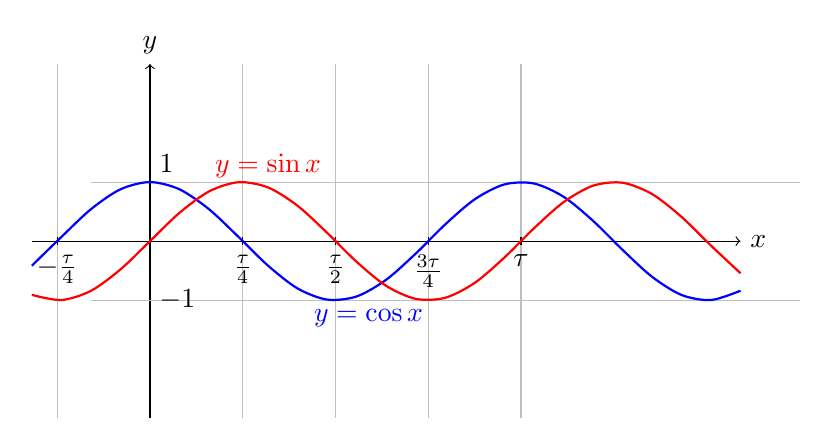
\begin{tikzpicture}[scale=0.75]
  \draw[->] (-2,0) -- (10,0) node[right] {$x$};
  \draw[->] (0,-3) -- (0,3) node[above] {$y$};
  \foreach \x/\xtext in
    {{pi/2}/{\frac \tau 4}, {pi}/{\frac \tau 2},
     {2*pi}/{\tau}, {3*pi/2}/{\frac {3\tau} 4}, {-pi/2}/{-\frac {\tau}{4}}} {
    \draw[shift={(\x,0)},lightgray] (0,-3) -- (0,3);
    \draw[shift={(\x,0)}] (0pt,2pt) -- (0pt,-2pt) node[below] {$\xtext$};
  }
  \foreach \y in {1, -1} {
    \draw[shift={(0,\y)},lightgray] (-1,0) -- (11,0);
  }
  \draw (0,1) node [above right] {$1$};
  \draw (0,-1) node [right] {$-1$};
  \draw[domain=-2:10,smooth,variable=\x,blue,thick] plot ({\x},{cos(deg(\x))});
  \draw[domain=-2:10,smooth,variable=\x,red,thick] plot ({\x},{sin(deg(\x))});
  \draw (3.7,-1) node[blue,below] {$y=\cos x$};
  \draw (2,0.9)  node[red,above] {$y=\sin x$};
  \end{tikzpicture}
  \caption{%
  The graphs of the functions $\sin$, $\cos$ of 
  a generic period $\tau$.}
\end{figure}